\documentclass{article}
\usepackage[utf8]{inputenc}
\usepackage[a4paper, total={7in, 9in}]{geometry} % Adjusted for smaller margins
\usepackage{hyperref}
\usepackage{amsmath}
\usepackage{amssymb}
\usepackage{graphicx}

\title{Reply to Editor and Reviewers}
\author{}
\date{\today}
% \usepackage[style=authoryear,giveninits=true,uniquename=init]{biblatex}
% Make parenthical citations the default
% \renewcommand\cite{\parencite}
% \addbibresource{refs.bib}

\usepackage{mwe}
\usepackage{blindtext}
\usepackage{natbib}
\usepackage{graphicx}
\usepackage{caption} % to get nicer top captions with tables
\usepackage{placeins}

%table commands
\usepackage[table]{xcolor}
\usepackage{makecell}
\usepackage{multirow}
\usepackage{tabularx}

\renewcommand{\cite}[1]{\citep{#1}}
\newcommand{\bluecline}[1]{\arrayrulecolor{blue}\cline{#1}\arrayrulecolor{black}}
\newcommand{\thickhline}{\Xhline{3.5\arrayrulewidth}}

\newcommand{\greencheck}{{\color{green}\checkmark}}

\newcommand{\miaojing}[1]{\textcolor{green}{[MS: #1]}} 
\newcommand{\tom}[1]{\textcolor{blue}{[TV: #1]}}
\newcommand{\tosin}[1]{\textcolor{magenta}{[TA: #1]}}

\newcommand{\secref}[1]{Section~\ref{#1}}


% to change the colour of text
\usepackage{xcolor}
% to strike through text
\usepackage[normalem]{ulem}
% to frame text
\usepackage{framed}

% to help with quoting added material in the revised paper 
\usepackage{quoting}
% \newcommand{\say}[1]{%
% \begin{quoting}
% #1
% \end{quoting}
% }

\newcommand{\sayold}[1]{%
{\color{olive}#1}
}



\newcommand{\saydel}[1]{%
{\color{darkgray}\sout{#1}}}

\newcommand{\saymod}[1]{%
  \texorpdfstring{\textcolor{blue}{#1}}{#1}%
}

% \newcommand{\saymod}[1]{#1}


\newcommand{\sayintro}[1]{%
  \texorpdfstring{\textcolor{olive}{#1}}{#1}%
}

\newcommand{\saynew}[1]{%
{\color{orange}#1}}

\newcommand{\reviewcomment}[3]{%
\vspace{4mm}
\textbf{C[$R_{#1}C_{#2}$]:} {\it #3}
\vspace{2mm}
}

\newcommand{\response}[1]{%
{\textbf{R:}} {#1}
}

% Change the default figure/table numbering to avoid confusion with main manuscript
\renewcommand{\figurename}{Fig.}
\renewcommand{\thefigure}{L\arabic{figure}}
\renewcommand{\thetable}{L\arabic{table}} 
\newcommand{\figref}[1]{\figurename~\ref{#1}}
\newcommand{\tabref}[1]{\tablename~\ref{#1}}
\newcommand{\subresponse}[1]{\underline{\MakeUppercase{#1}}}
% \newcommand{\enclose}[1]{\par\indent """  #1   \indent """\par}

\newcommand{\enclose}[1]{%
%    \smallskip
%    \par
%    \noindent%
%    \fbox{%
%        \begin{minipage}{\dimexpr\linewidth-2\fboxsep-2\fboxrule\relax}#1 
%        \end{minipage}%
%    }%
%    \par
\begin{framed}
#1
\end{framed}
}

% \usepackage[pdfusetitle,hidelinks]{hyperref}

\begin{document}

\maketitle

In the revised document that we join with this reply, the deleted old parts are in \saydel{striked out dark gray}, the modified parts in \saymod{blue}
and the added parts in \saynew{orange}.
%
Changes made to the revised manuscript and reproduced in this letter for ease of use are highlighted using a simple frame as:
\enclose{Text from revised document.}


%%%
\section{Detailed Answer to Editor's comments}


\reviewcomment{E}{1}{
Please remove the URL from the Abstract
}

\response{
It has been removed.   

\enclose{
CholecInstanceSeg aims to advance the field by offering a comprehensive and high-quality open-access dataset for the development and evaluation of tool instance segmentation algorithms. 
\saydel{CholecInstanceSeg is publicly available \href{https://www.synapse.org/Synapse:syn60239970/wiki/628710}{here}}
}

}

\reviewcomment{E}{2}{
While I appreciate that you did not collect the original dataset yourself, I was unable to find appropriate ethical approvals and consent for data publication for the Cholec datasets. 
While it would be fine to provide annotation of these data, we would not allow any reproduction of the dataset images / or surgical frames from these data in this work unless we could confirm that not only was ethical approval acquired for the original dataset, but that consent was acquired for the publication of the data. If this was obtained by the original authors, please make sure to direct us to this information, otherwise, if you would like to continue with this submission, please do the following:

%}

%\reviewcomment{E}{2i}{
\emph{\textbf{C[$R_{E}C_{2i}$]:}}
Please remove all images / surgical stills from the repository. The only thing that should remain are any annotations that you have generated. Please also remove the stills from the figures of this work.

}

\response{
We have removed all surgical stills from the repository, leaving only the annotations we generated. In the manuscript, we have also removed all figures containing stills and made corresponding modifications to the text where these figures were referenced.
%
Additionally, we have removed the supplementary material, as it primarily contained explanations on how we annotated hard cases using surgical stills. 
%We will be including a note in the rebuttal email requesting its removal from the submission.
%
The following deletions have been made in the manuscript:

\enclose{
\saydel{A visual representation of these tool categories is shown in \figref{fig:tools}} 
}

\enclose{
\saydel{A clear visual representation of this unique situation with the instrument port can be seen in \figref{fig:instrument_port}}
}

\enclose{
 \saydel{A visual representation of these hard cases can be seen in \figref{fig:hard_cases}.  More detailed information about specialized instructions given to annotators for hard cases is added as supplementary material for this manuscript.} 
}



}

\reviewcomment{E}{2ii}{
Please relabel all files so that the provenance of the images/surgical frames is noted, with enough detail that readers will be able to combine your annotations to the original files.

}

\response{
All the annotations files are currently organised and labelled with enough details such that readers can easily combine the annotations with the original files. 

}

\reviewcomment{E}{2iii}{
Please generate a file that provides all metadata of the original dataset, combined with the organization of your annotations, so that readers will be able to see at a glance how your annotations correspond to the original dataset and can more easily link the datasets.

}

\response{
We included a metadata file   $cholecinstanceseg\_metadata.csv$  in the dataset repository.  The metadata file is a comma separated value file with information on each annotation files such as the annotation filename, image filename in the source dataset, video id, dataset split, source dataset, and annotation path. 
%
In addition, we mention the metadata file in the data records section of the original manuscript. 

\enclose{


\saynew{The metadata file $cholecinstanceseg\_metadata.csv$ provides additional information about each annotation, including the annotation filename, corresponding image filename in the source dataset, video ID, dataset partition (train, val, or test), source dataset, and the annotation file path. This metadata enables researchers to link CholecInstanceSeg annotations with the original datasets.}


}


}

\reviewcomment{E}{2iv}{
 Please confirm in your response letter that you have removed all images/surgical frames from the repository.
}

\response{
All images/surgical frames have been removed from the dataset repository which accompanies this manuscript. 
}

\reviewcomment{E}{2v}{
 Please change the data licence to CC0 or CC-BY at the repository wiki, modifying any other descriptions (such as license files or comments in the paper) to match
}


\response{
The data licence at the wiki has been changed to CC-BY. The following statement has been added to the dataset repository 

\enclose{
This work is licensed under a  Creative Commons Attribution 4.0 International License \href{ https://creativecommons.org/licenses/by/4.0/}{(CC BY 4.0)} 
}
}



\reviewcomment{E}{3}{
Because at least some of your data looks to originate from third parties, please check the following and confirm/state what has been done in your ‘response to reviewers’ document.

%}

%\reviewcomment{E}{3i}{
%\emph{\textbf{C[$R_{E}C_{3i}$]:}}
Ensure all sources are clearly described in the main text. For general mentions of services, databases, or other platforms, please name the resource in the main text and provide a URL in () s. Instructions should be sufficient for the exact input data to be retrieved, so please provide specific links, accession numbers, or the exact search term/query when discussing any data from general databases. For specific datasets downloaded from repositories, or other items with formal metadata, please use a full citation in the reference list containing the relevant DOI. Note this should be the dataset, rather than any relevant publication, however these should be cited as well if required, or if the data was newly extracted from a document.
}

\response{
All data sources are explicitly described in the main text with entire subsections dedicated to descriptions of source datasets. The exact URLs for downloading the source datasets have been provided in the Data Records section. Additionally, metadata information to enable users combine our dataset with the source dataset has been included and explained in the manuscript. Utility python scripts to facilitate integration of the source datasets with our annotations to have been made available, which is mentioned in the Code Availability section.

Regarding citations, the datasets used do not have assigned DOIs. Instead, their original authors request that users cite the corresponding publication references rather than a dataset-specific DOI. Therefore, we have cited the official publications associated with each dataset, in accordance with the dataset providers' guidelines.
}

\reviewcomment{E}{3i}{
Confirm all the sources are openly available - i.e. your re-use or re-distribution is compliant with the terms and conditions/licenses for data sharing. If you cannot see a fully open license at the source, please check with the data provider. Please note it is your legal responsibility to ensure all data have been used or re-distributed appropriately and we cannot support publication of descriptions of data obtained or re-shared without this check
}



\response{
The Cholec80 and CholecT50 datasets (which we do not redistribute anymore but only provide a link to) are publicly available under the CC-BY-NC-SA 4.0 license. To ensure compliance with data sharing policies, we reached out to the dataset provider for clarification. We have received confirmation that we are permitted to share our annotations under our choice of license.
}


\reviewcomment{E}{8}{
Please add a data citation for the dataset to the reference list using these instructions. Note that a DOI URL should be used. 
Please add the reference number to wherever the dataset is mentioned in the text - the main position should be the first part of the Data Record in a sentence describing where the data has been deposited.
}

\response{
We have added the required data citation, including the DOI URL, to the reference list following the provided instructions. The dataset is now referenced in the first part of the Data Records section, as requested. Its reference number is 21 in the main manuscript.

\enclose{
\saynew{The CholecInstanceSeg dataset \cite{cholecinstanceseg} is publicly available.
}
}
}


\reviewcomment{E}{9}{
Please remove the current Data Record section and replace it with a description of the files being shared. This should include an opening sentence such as “The dataset is available at [name of repository]” followed by a practical description of the files (lines 279-293), including file names and folder structure (where these are not obvious or simple) and a description of column headings or variable names (where not implicit). No other content, such as a statistical summary of the data, should be included.
}

\response{
As requested, we have replaced the existing Data Records section with a structured description of the shared files. The revised section begins with a citation to the dataset repository, following Scientific Data standards, and provides a detailed breakdown of the dataset’s organization, file formats, and annotation structure.
%
Since the dataset does not contain column headings or variable names, we describe the folder structure, file formats, and metadata instead. Statistical summaries and analysis have been moved to the Technical Validation section, as they help to showcase the technical quality of our work, and can be used as reference for users.
%
We have also corrected our diagram showing the dataset folders, and subfolders, removing folders that contain images. 
%
The revised Data Records section now reads:


\enclose{

\saynew{%
\section*{Data Records}
The CholecInstanceSeg dataset \cite{cholecinstanceseg} is publicly available. Cholec80 and CholecT50 video frames used to generate the dataset can be obtained from the CAMMA research group website(\href{http://camma.u-strasbg.fr/datasets}{http://camma.u-strasbg.fr/datasets}). CholecSeg8k can be obtained at (\href{https://www.kaggle.com/datasets/newslab/cholecseg8k_cis}{https://www.kaggle.com/datasets/newslab/cholecseg8k_cis}).
%}



%\saynew{
The dataset is provided as a single archive, $CholecInstanceSeg.zip$, which contains the instance segmentation annotation files in $cholecinstanceseg.zip$ and a metadata file $cholecinstanceseg\_metadata.csv$ that provides metadata information about each annotation file and can be used to link each file to its source dataset. The annotation files are structured into two main directories: train and val, each containing individual video sequence folders. Each sequence folder includes an $ann\_dir$ subdirectory that stores instance segmentation annotations in JSON format. The test directory is withheld for benchmarking purposes and potential competition use, but it is available upon request.
%
A schematic representation of the dataset folder structure and a sample JSON annotation file are shown in \figref{fig:file_format}
%}

%\saynew{
Annotations are formatted following the LabelMe convention. Each shape is listed under the $shapes$ key, with a $label$ field specifying the instrument class, $points$ containing the (x, y) coordinates of the polygon defining the object’s boundary, $group\_id$ indicating the instance ID, $image\_Height$ for the height of image annotated and $image\_Width$ for its width.
}


}

\begin{figure}[ht]
  \centering
   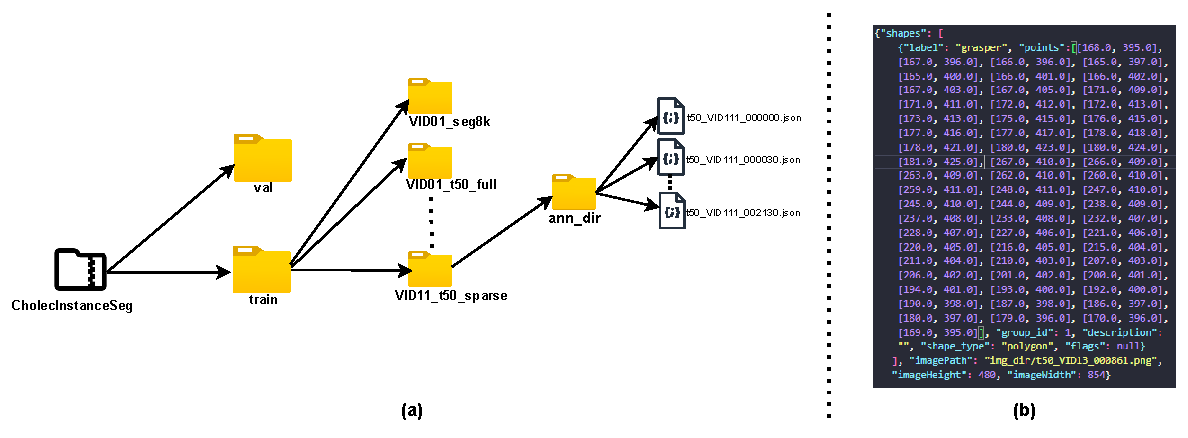
\includegraphics[width=\linewidth]{imgs/file_folder_structure_and_annotation_format.pdf}
   \caption{\saymod{(a) Dataset directory structure for CholecInstanceSeg. Each split (e.g. train) contains subdirectories for each sequence, with \saydel{subdirectories for images ($img\_dir$) and} further subdirectories for annotations ($ann\_dir$). (b) Sample JSON annotation file showing the structure of the annotation data, including class labels ("$label$"), polygon information ("$points$")  and instance IDs ("$group\_id$").}}
   \label{fig:file_format}
\end{figure}

}

\reviewcomment{E}{10}{
Please remove the current usage notes section, as only providing annotations does not require a CC-BY-NC-SA license and standard academic convention means that authors will cite your work if they use it.
}

\response{
The usage notes section has been removed. 
}




\section{Detailed Answer to Reviewer 1}

We thank you for your careful reading of our manuscript and your encouraging comments.  

\reviewcomment{1}{1}{
Introduction: It would be useful to describe cholecystectomy in more detail, which objects in the images are of importance, the need for segmentation (there is only one gallbladder), etc. Describe how detecting various objects in video during surgery can be beneficial. \hypertarget{1_1}{}
}

\response{
We appreciate the reviewer’s suggestion to provide more context into Cholecystectomy and instance segmentation.
To address this, we have expanded the introduction to include a description of the laparoscopic cholecystectomy procedure and the relevance of instance segmentation specifically instrument instance segmentation.
%
We now further discuss the importance of detecting surgical instruments, emphasizing their role in understanding surgical scenes and enabling downstream tasks in computer-aided interventions.


\enclose{
Minimally invasive surgeries (MIS) have gained popularity due to their benefits over open surgeries, such as reduced blood loss, less pain, faster recovery times, and fewer post-surgical complications~\cite{fuchs2002minimally}. However, MIS relies on an endoscope or laparoscope for indirect vision, which provides a limited field of view, making it challenging for surgeons to accurately interpret complex surgical scenes ~\cite{real_time_seg_adverserial_cis}. To overcome this, computer-aided intervention techniques that enhance the information obtained through minimally invasive cameras have been proposed~\cite{vecauteren_cai_4_cai_cis,cv_in_surgery_cis}.
At the forefront of this evolution lies the challenge of achieving precise instance segmentation of surgical tools in a minimally invasive surgical scene.
\saydel{This task is essential for developing assistive surgical technology and autonomous or semi-autonomous surgical systems, which require detailed knowledge of the identification and localization of various tools.}
\saynew{Detecting and segmenting instances of these instruments is critical to enhance surgical scene understanding, track instrument interactions, and support downstream tasks such as surgical workflow recognition, skill assessment and surgical training, augmented reality overlays, safety and error detection,  and autonomous assistance systems.}

Current publicly available datasets for surgical tool segmentation have several notable limitations.
Many focus on porcine or ex-vivo surgeries rather than routine human procedures, limiting their applicability to day-to-day clinical settings~\cite{endovis2015,endovis2017_cis,endovis2018_cis}.
Others are multitask datasets with limited tool segmentation data~\cite{autolaparo_cis}, or they provide only binary instance segmentation for a single tool class~\cite{robustmis2019_cis}. Additionally, available surgical tool segmentation datasets lack instance-specific information ~\cite{endovis2015,endovis2017_cis,endovis2018_cis,autolaparo_cis,psychogyios2023sar_cis,cholecseg8k_cis}, and most offer a relatively small number of annotated segmentation masks. 
%typically fewer than 10,000~\cite{endovis2017_cis,endovis2018_cis}.


\saydel{To overcome these challenges, we introduce the CholecInstanceSeg open-access dataset, in which we meticulously annotate 41,933 frames extracted from 85 laparoscopic cholecystectomy procedures from the existing Cholec80 \mbox{~\cite{endonet_cis}}
 and CholecT50 \mbox{~\cite{NWOYE2022102433_rendevous_cis}} datasets.}

To overcome these challenges, we introduce the CholecInstanceSeg open-access dataset, in which we meticulously annotate 41,933 frames from the existing Cholec80~\cite{endonet_cis} and CholecT50~\cite{NWOYE2022102433_rendevous_cis} datasets \saynew{with instance segmentation labels and class labels for 7 instrument classes: Grasper, Bipolar, Hook, Clipper, Scissors, Irrigator, and Snare. 
CholecInstanceSeg contains frames from 85 videos of Laparoscopic cholecystectomy - a routine surgical procedure for gallbladder removal, commonly performed to treat gallstones or cholecystitis. It is the most common MIS procedure, accounting for approximately a quarter of all MIS procedures~\citep{MATTINGLY202333}.}


}

}



% \enclose{

% Minimally invasive surgeries (MIS) have gained popularity due to their benefits over open surgeries, such as reduced blood loss, less pain, faster recovery times, and fewer post-surgical complications~\cite{fuchs2002minimally}.
% \saydel{However, MIS relies on an endoscope or laparoscope for indirect vision, which provides a limited field of view, making it challenging for surgeons to accurately interpret complex surgical scenes ~\cite{real_time_seg_adverserial_cis}. }
% \saynew{However, MIS presents numerous challenges for accurate scene interpretation, including limited visual perspective, poor lighting, occlusions, quick motions, and the presence of fluid ~\cite{real_time_seg_adverserial_cis,vecauteren_cai_4_cai_cis,cv_in_surgery_cis}. 
% }

% \saynew{An example of MIS is laparoscopic cholecystectomy, a routine surgical procedure for gallbladder removal, commonly performed to treat gallstones or cholecystitis. In the United States alone, approximately 300,000 cholecystectomies are performed annually \citep{hassler2023laparoscopic}. The procedure requires the use of multiple surgical instruments such as graspers, hooks, and scissors within a constrained workspace. Detecting and segmenting instances of these instruments is critical to enhance scene understanding, track instrument interactions, and support downstream tasks such as surgical workflow recognition, skill assessment, augmented reality overlays, and autonomous assistance systems. 
% }

% To overcome \saydel{this,} 
% \saynew{several challenges for accurate surgical scene interpretation, computer-aided intervention techniques that enhance the information obtained through minimally invasive cameras have been proposed ~\cite{vecauteren_cai_4_cai_cis,cv_in_surgery_cis}. At the forefront of this evolution lies the challenge of achieving precise instance segmentation of surgical tools in a minimally invasive surgical scene.
% This task is essential for developing assistive surgical technology and autonomous or semi-autonomous surgical systems, which require detailed knowledge of the identification and localization of various tools.

% }

% }
% }



\reviewcomment{1}{2}{
Introduction:  Provide more context for the details of the study such as the number and types of classes chosen.
}

\response{
We thank the reviewer for their comment.
The names, descriptions, diagrams, rationale for the instrument choices, and additional context for the study are provided in the Labelling Protocol section of the manuscript. However, in response to the reviewer’s suggestion, we have included key details about the number and types of classes directly in the introduction.

\enclose{
To overcome these challenges, we introduce the CholecInstanceSeg open-access dataset, in which we meticulously annotate 41,933 frames from the existing Cholec80~\cite{endonet_cis} and CholecT50~\cite{NWOYE2022102433_rendevous_cis} datasets \saynew{with instance segmentation labels and class labels for 7 instrument classes: Grasper, Bipolar, Hook, Clipper, Scissors, Irrigator, and Snare. 
CholecInstanceSeg contains frames from 85 videos of Laparoscopic cholecystectomy - a routine surgical procedure for gallbladder removal, commonly performed to treat gallstones or cholecystitis. It is the most common minimally invasive surgery (MIS) procedure, accounting for approximately a quarter of all MIS procedures~\citep{MATTINGLY202333}.}
}
}


\reviewcomment{1}{3}{
Introduction:  Also provide an overview of deep learning methodologies used in the past, accuracies achieved, limitations, etc. \hypertarget{1_3}{}
}

\response{
We appreciate the reviewer’s comment. 
%However, 
As the primary aim of the paper is to introduce CholecInstanceSeg as a dataset descriptor, an in-depth review of past deep learning methodologies is beyond its scope. We have instead added a reference to a recent review paper  \citep{rueckert2024methods} in the introduction for readers that might be interested in learning more about methods and how they relate to datasets. 

\enclose{
Minimally invasive surgeries (MIS) have gained popularity due to their benefits over open surgeries, such as reduced blood loss, less pain, faster recovery times, and fewer post-surgical complications~\cite{fuchs2002minimally}. However, MIS relies on an endoscope or laparoscope for indirect vision, which provides a limited field of view, making it challenging for surgeons to accurately interpret complex surgical scenes ~\cite{real_time_seg_adverserial_cis}. To overcome this, computer-aided intervention techniques that enhance the information obtained through minimally invasive cameras have been proposed~\cite{vecauteren_cai_4_cai_cis,cv_in_surgery_cis}.
At the forefront of this evolution lies the challenge of achieving precise instance segmentation of surgical tools in a minimally invasive surgical scene.
\saydel{This task is essential for developing assistive surgical technology and autonomous or semi-autonomous surgical systems, which require detailed knowledge of the identification and localization of various tools.}
\saynew{Detecting and segmenting instances of these instruments is critical to enhance surgical scene understanding, track instrument interactions, and support downstream tasks such as surgical workflow recognition, skill assessment and surgical training, augmented reality overlays, safety and error detection,  and autonomous assistance systems.}
\saynew{Surgical instrument segmentation is an active field of research which has been significantly advanced by use of deep learning techniques for single-frame detection and temporally-aware methods. This progress is comprehensively reviewed in \cite{rueckert2024methods}, which provides a detailed overview of the current state of research and highlights key advancements in the field.}
}



}



\reviewcomment{1}{4}{
Data source: It would be great to provide subject characteristics, severity of the diseases, etc.
}

\response{
While we acknowledge that it would be relevant,
this information is not provided for the Cholec80 or CholecT50 datasets, from which the frames are derived. 
We are thus not in a position to add this information to our manuscript.
}

\reviewcomment{1}{5}{
Data source:  Provide technical specifications for the images and videos, field of view, spatial resolution, etc.  Provide details on data pre-processing methodology (from video to image). \hypertarget{technical_specs}{}
}

\response{
We thank the reviewer for this suggestion. While the technical specifications were partially described in the \emph{File format} section, we have now reiterated and expanded this information in the data sources section for clarity. Specifically, we have added details about the resolution, field of view, and frame extraction process used to generate the dataset.


\enclose{
When discussing the source datasets, we distinguish between videos and image sequences. Videos are multimedia compressed files provided in formats such as .mp4, while image sequences refer to extracted sequential frames from videos. 

\saynew{The frames from Cholec80 and CholecT50 used in CholecInstanceSeg are primarily at a resolution of 854x480 pixels, consistent with the original Cholec80 and CholecT50 datasets. However, three sequences from CholecT50 are provided at a higher resolution of 1920x1080 pixels. CholecT50 contains pre-extracted image sequences and we used these as is, while frames from Cholec80 were extracted at 1 fps using the FFMPEG library.}}
}

\begin{figure}[ht]
  \centering
  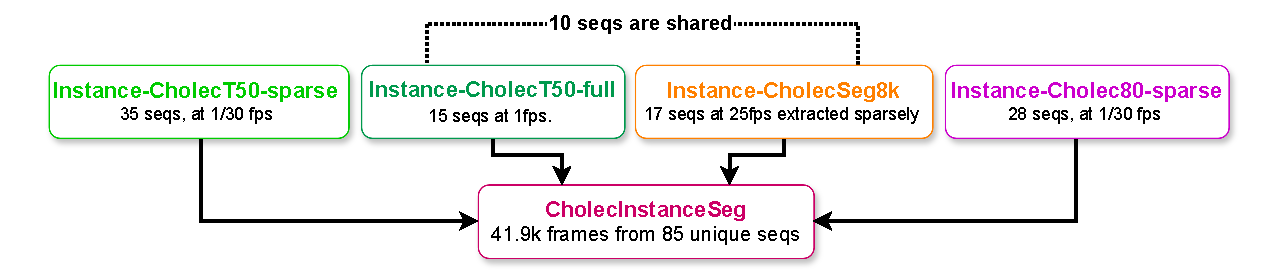
\includegraphics[width=\linewidth]{imgs/cholec_instance_seg_map.pdf}
   \caption{CholecInstanceSeg is composed of frames from four dataset partitions: Instance-CholecT50-sparse, Instance-CholecT50-full, Instance-CholecSeg8k, and Instance-Cholec80-sparse. The diagram illustrates the number of image sequences (denoted \emph{seqs} in the figure for brevity) and extraction rates for each partition. Note that 10 sequences are shared between Instance-CholecT50-full and Instance-CholecSeg8k.}
   \label{fig:our_dataset} 
\end{figure}

\begin{figure}[ht]
\centering
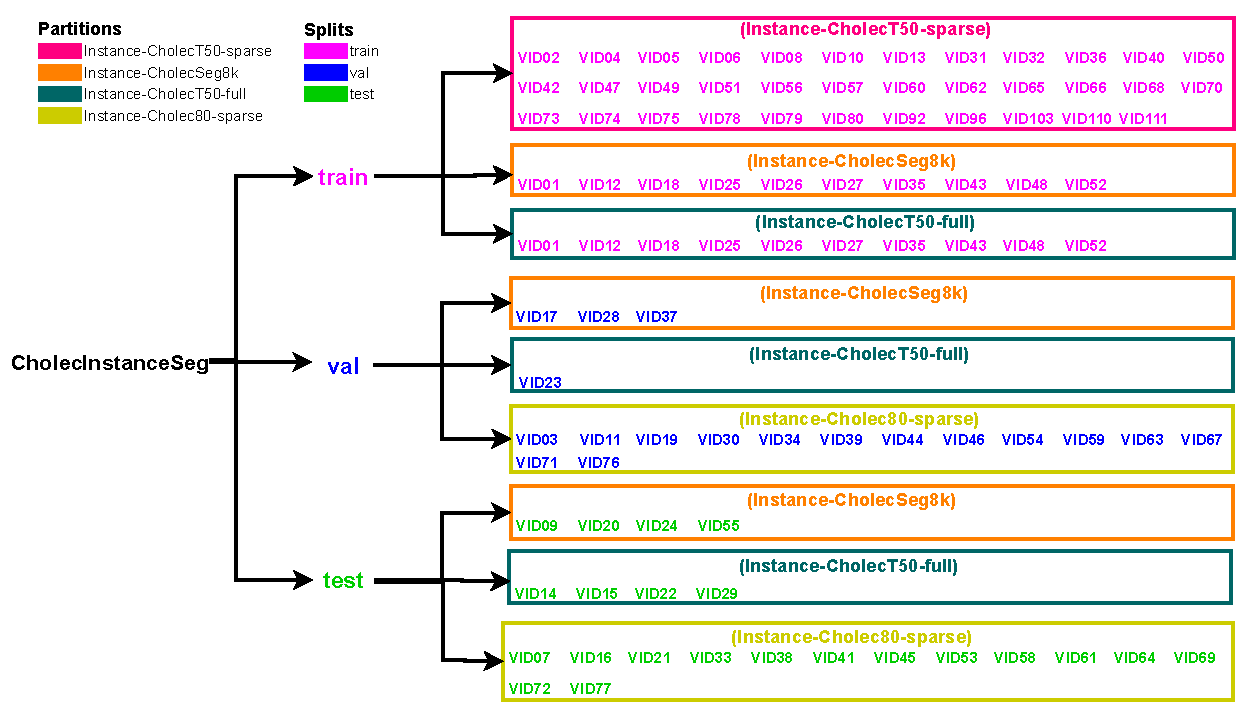
\includegraphics[width=\linewidth]{imgs/train_test_split_dataset_partitions.pdf}
\caption{Recommended dataset splits for CholecInstanceSeg. The diagram shows the distribution of sequences across the training, validation, and testing datasets, highlighting the specific partitions (Instance-CholecT50-sparse, Instance-CholecSeg8k, Instance-CholecT50-full, Instance-Cholec80-sparse) and their corresponding sequences.}
\label{fig:recommended_dataset_splits}
\end{figure}


\reviewcomment{1}{6}{
Data source: There was a lot of discussion on different frames per seconds issue when analyzing different datasets, but the importance of this is not clearly articulated? 
}

\response{
We thank the reviewer for highlighting this point. The differences in frame rates across the dataset partitions stem from two key factors: 1) the design of the parent datasets -- Cholec80 provides videos at 25fps which we then extract at 1fps and CholecT50 provides image sequences at 1fps directly --; and 2) the practical constraints associated with annotating sequences. 
Annotating every image sequences at 1fps is prohibitively expensive, so we employed a mixed approach by annotating some sequences \emph{fully} (using all available frames at 1fps) and others \emph{sparsely} (sampling frames at a further reduced framerate of $\frac{1}{30}$ fps). This approach balances annotation density with dataset diversity. We have clarified this rationale in the manuscript and explained the implications for annotation and dataset coverage.



\enclose{
\subsubsection*{Summary of CholecInstanceSeg Partitions}
CholecInstanceSeg, which contains 41.9k frames from 85 unique image sequences, can be partitioned into four distinct sections based on the data source: Instance-CholecSeg8k, Instance-CholecT50-full, Instance-CholecT50-sparse, and Instance-Cholec80-sparse. \saynew{Our process for selecting the frames and sequences for each partition is as follows:}
%
\begin{enumerate}
    \item Instance-CholecSeg8k: \saymod{We selected} all the 8,080 frames from all the 17 sequences provided in CholecSeg8k, we utilized all the images in CholecSeg8k.
    \item Instance-CholecT50-full: \saymod{We randomly selected}  15 sequences within CholecT50 (CholecT50-full), we utilized all frames provided by CholecT50 for these \saynew{15} sequences \saynew{- 28,317 frames}.
    \item Instance-CholecT50-sparse: For the remaining 35 \saynew{(50-15)} sequences in CholecT50(CholecT50-sparse), we sampled these sequences by selecting one frame out of every 30 frames ($\frac{1}{30}$ fps), ensuring a minimum of 50 frames in each sequence \saynew{- 2,681 frames} . 
    \item Instance-Cholec80-sparse: \saymod{After selecting sequences for Instance-CholecSeg8k, Instance-CholecT50 (both full and sparse),} there remained 28 videos from Cholec80, which are not included in CholecT50 and CholecSeg8k, and these videos were sampled at $\frac{1}{30}$ fps, ensuring a minimum of 50 frames in each sequence \saynew{- 2,855 frames} . 
\end{enumerate}
%


A visual representation of dataset partitions in CholecInstanceSeg can be seen in \figref{fig:our_dataset}. 
\saynew{
The differences in frame rates for each dataset partition reflect both the design of the parent datasets -- Cholec80 provides videos at 25fps which we then extract at 1fps and CholecT50 provides image sequences at 1fps directly -- and practical considerations for annotating instance segmentation on a large number of frames. Annotating every sequence densely at 1fps is prohibitively expensive. Thus, we adopted a mixed approach, converting existing semantic segmentation to instance segmentation, annotating some sequences \emph{fully} (using all frames available from the parent datasets), and others sparsely (sampling frames at reduced frame rates of $\frac{1}{30}$ fps). This approach allows us to balance annotation density and dataset diversity, ensuring coverage of both densely annotated sequences and a wider range of surgical scenes.

\figref{fig:recommended_dataset_splits} presents the exact sequences in each partition, represented as VID-XX, where XX is the sequence number. 
}
}

}


\reviewcomment{1}{7}{
Data source:  Additionally, it is not clear if each dataset was acquired using different equipment, and if there are obvious differences in quality or characteristics of the images from each dataset. \hypertarget{1_7}{}
}

\response{
We thank the reviewer for raising this point. All datasets used in CholecInstanceSeg (Cholec80, CholecT50, and CholecSeg8k) were collected by the CAMMA research group and are publicly available subsets of the in-house Cholec120 dataset. These datasets were recorded at the University Hospital of Strasbourg. While they were released in different formats (videos or frames) and annotated for different tasks, the exact acquisition equipment used for each video or each released dataset was not specified in the original datasets.
We are thus not in a position to add specific information about surgical equipment to our manuscript.

There are no significant differences in video quality across the datasets, except for a resolution change observed in three videos, which we have noted in the manuscript as a response to \hyperlink{technical_specs}{\textbf{$R_{1}C_{5}$}} . We have added the information about the data being recorded at the University Hospital of Strasbourg to the manuscript, as this was not previously specified.


\enclose{
The CholecInstanceSeg dataset is curated using frames extracted from three existing laparoscopic cholecystectomy datasets: Cholec80 \cite{endonet_cis}, CholecT50 \cite{NWOYE2022102433_rendevous_cis}, and CholecSeg8k \cite{cholecseg8k_cis}, containing a total of 85 image sequences.
These datasets are publicly available subsets of the in-house Cholec120 dataset \cite{twinanda2018rsdnet_cis} from the CAMMA research group \saynew{which was recorded at the University Hospital of Strasbourg \cite{endonet_cis,NWOYE2022102433_rendevous_cis}}. 
}
 }


\reviewcomment{1}{8}{
Labelling: as mentioned above, rationale for detecting different objects/tissues should be more clear. For example, there are 7 categories for the tools, which seems to be least important objects to categorize (wouldn't the surgeon or robot already know which tools are being used and the location/position of the tools?)
\hypertarget{1_8}{} }

\response{
We thank the reviewer for this insightful comment and the opportunity to clarify the rationale for detecting and categorizing surgical tools. 
%
CholecInstanceSeg focuses on a (non-robotic) laparoscopic cholecystectomy use case.
While the surgeons do not require any assistance in identifying the tools, a computationally tractable understanding of the position of tools and their interaction within the surgical scene is needed to design downstream surgical assistance (e.g. surgical workflow recognition, AR overlays, etc.).
%
Even in the context of robotic surgery (which we do not cover in this manuscript), a number of factors such as the use of extra non-robotic instruments, slack in robot kinematics and cumbersome camera calibration steps lead to an imprecise knowledge of surgical tool positions in image space. This makes surgical tool segmentation a relevant building block in all forms of minimally invasive surgery.

%While it may seem that the type and position of tools are inherently known, this is not the case in laparoscopic surgery especially tranditional laparoscopic surgery.
%In traditional laparoscopic procedures, surgeons perform the surgeries manually, relying on indirect vision through a laparoscope. The precise positions and interactions of tools with tissues are not available and must be interpreted visually. 
%Traditional laparoscopic surgery differs from robotic-assisted laparoscopic surgery, but even in robotic systems, tool instance segmentation remains crucial. In robotic laparoscopic surgery, while the robotic system may have information about the tools it manipulates, this data often lacks spatial context within the surgical scene. Tool instance segmentation provides visual information to accurately localize the tools and support downstream applications for computer-aided interventions such as: tool tracking,  surgical workflow recognition, skill assessment and surgical training, Augmented Reality Overlays, Safety and Error Detection, Autonomous Assistance Systems. 

We have updated the `Background and Summary' section to emphasize the importance of surgical tool instance segmentation and added a reference to a recent review paper to highlight that surgical instrument segmentation is an active area of research. 

% In addition, we have added a new subsection called `Downstream applications' were we further explain how tool instance segmentation advances key downstream tasks.   


\enclose{
\saynew{Detecting and segmenting instances of these instruments is critical to enhance surgical scene understanding, and supporting downstream tasks such as tool tracking,  surgical workflow recognition, skill assessment and surgical training, augmented reality overlays, safety and error detection,  and autonomous assistance systems.}
\saynew{Surgical instrument segmentation is an active field of research which has been significantly advanced by use of deep learning techniques for single-frame detection and temporally-aware methods. This progress is comprehensively reviewed in \cite{rueckert2024methods}, which provides a detailed overview of the current state of research and highlights key advancements in the field.}
}

% \enclose{
% \subsection*{\saynew{Downstream Applications}}
% \saynew{The CholecInstanceSeg dataset offers significant potential for advancing various downstream applications beyond segmentation. Key downstream tasks include:

% \begin{itemize}
%     \item Tool tracking: accurate surgical tool instance segmentation is a critical precursor for tool tracking algorithms. By enabling precise localization and motion analysis of each tool across frames, it facilitates applications such as trajectory prediction, and motion planning. 
%     \item Surgical workflow recognition: surgical tool instance segmentation data supports workflow recognition by identifying tools in use and determining their interactions with anatomical structures. This application can improve intraoperative decision-making and provide valuable insights for post-surgical analysis.
%     \item Skill assessment and surgical training: tool instance segmentation annotations aid in the identifying tools, tracking interactions, analyzing tool paths and trajectories, recognizing gestures, and measuring positional accuracy. These capabilities are critical for evaluating surgical skill and improving surgical training.  
%     \item Augmented reality overlays: tool instance segmentation enables precise detection, localization, and tracking of instruments, ensuring that augmented reality overlays are accurate. This supports guidance systems that rely on overlays and ensures they are correctly updated.
%     \item Safety and error detection: tool instance segmentation facilitates monitoring of tool-tissue interactions to prevent adverse events, such as tool misalignment or prolonged tissue contact. For laparoscopic cholecystectomy, it can jelp in addressing the critical view of safety challenge, reducing the risk of bile duct injury.  
%     \item Autonomous assistance systems: tool instance segmentation data can inform autonomous systems for automatic tool manipulation, multi-tool coordination and planning and other tasks required for autonomous assistance.
% \end{itemize}

% }

% }


% \response{
% We thank the reviewer for this insightful comment and the opportunity to clarify the rationale for detecting and categorizing surgical tools. While it may seem that the tool type and position are inherently known, this assumption does not hold for all real-world scenarios, particularly for downstream applications in computer-aided interventions.

% We have updated the `background and summary' section to emphasize the importance of surgical tool instance segmentation.

% \enclose{\saynew{Surgical tool segmentation, particularly instance segmentation, is essential for enabling downstream tasks critical to advancing surgical care. Precise localization and categorization of tools facilitate workflow recognition, real-time decision-making in robotic surgeries, skill evaluation, visual servoing tasks, surgical training, as well as determining safety in the interaction of tools with tissues. These capabilities demonstrate the indispensable role of tool instance segmentation in modern computer-aided intervention systems.}}

% }
}


\reviewcomment{1}{9}{
Labelling:  on the contrary, wouldn't it be important to detect individual clips, needles, and sutures, to determine that the ducts and vessels are properly sealed? It would seem important to know if there's a stray clip/needle/suture...
}

\response{
We agree with the reviewer that detecting individual clips, needles, and sutures is an important aspect of ensuring surgical safety and evaluating procedural outcomes.
Essentially, the more refined the visual understanding of the surgical scene, the more downstream applications we can envision supporting. 
However, as detailed in our previous responses \hyperlink{1_1}{\textbf{$R_{1}C_{1}$}}, \hyperlink{1_3}{\textbf{$R_{1}C_{3}$}}, and 
\hyperlink{1_8}{\textbf{$R_{1}C_{8}$}}, the focus of this study is on surgical tool instance segmentation, specifically the localization and identification of primary surgical instruments (e.g., graspers, hooks, scissors). 
%
We believe that our current statement about the \emph{Annotation scope}, reproduced below for simplicity, already captures our rationale. We believe CholecInstanceSeg already provides a significant advance for the field.

\enclose{
\subsubsection*{Annotation scope}
The annotation scope defines the entities included and excluded to maintain a focused and high-quality dataset. While we annotated all laparoscopic tools,  some objects used in conjunction with these tools were excluded to streamline the annotation process:
%
\begin{itemize}
    \item Excluded Entities: Individual clips from the clipper, surgical needles, surgical sutures, the specimen bag, the camera port, and gauze. 
\end{itemize}    
}

}

\reviewcomment{1}{10}{
Annotation:  a validation step is needed to show how accurately SAM captured the intended area, vs. a manual segmentation by an expert. This key step must be performed on selected subset of the data to determine if the SAM segmentation accuracy is sufficiently high. This is a major weakness of this study that must be addressed. 
Related, it is not clear what kind of accuracy is needed / targeted.
}

\response{
We thank the reviewer for highlighting the importance of validating the accuracy of SAM-generated segmentations compared to manual annotations. This validation step is already included in the Technical Validation section of the manuscript (partially reproduced below for ease of reading), where we performed a Manual vs. Semi-automatic Validation. Specifically, we measured the agreement between manual annotations and SAM-assisted annotations using the Panoptic Quality Metric. 


\enclose{
\subsubsection*{Manual vs Semi-automatic Agreement}
To validate the consistency of our semi-automatic annotation pipeline against the manual annotation process, we measured the agreement between the two methods using the Panoptic Quality Metric. This comparison was crucial to ensure that the increased speed of the semi-automatic pipeline did not compromise annotation quality. The results demonstrated a high level of agreement, with a Panoptic Quality score of 95.7, indicating that the semi-automatic annotations were consistent with the manual annotations.
}

}

\reviewcomment{1}{11}{
Annotation:  on a similar note, there is now medical SAM that may perform much better than SAM.
}

\response{We appreciate the reviewer’s comment and acknowledge the advancements in tools such as MedSAM \citep{ma2024segment}. However, at the time this project began, MedSAM was not yet available. The original SAM sufficiently met the requirements of our workflow, enabling us to efficiently and accurately generate annotations for the dataset. This was validated through the high Panoptic Quality score (95.7) achieved in our manual vs. semi-automatic agreement evaluation.
%
Future iterations of CholecInstanceSeg or similar projects may explore the use of MedSAM to assess whether it can further enhance the annotation process.}

\reviewcomment{1}{12}{
Annotation:   conversion of semantic to instance segmentation is a clever time-saver!
}

\response{
We appreciate the reviewer’s recognition of this approach as an effective time-saver. 
}

\reviewcomment{1}{13}{
Annotation:  semi-automatic annotation: it is not clear how the errors were corrected; was SAM used to provide a whole-new annotation?
}

\response{
We appreciate the reviewer’s comment and the opportunity to clarify the error correction process in our semi-automatic annotation pipeline. Errors were addressed depending on the severity of the error. 
% situationally 
% leveraging both the SAM model and traditional annotation tools integrated into our workflow. 
Specifically, when only small adjustments were needed, we used the contour correction tools available in the LabelMe annotation platform. 
For significant inaccuracies or when new annotations were required, SAM’s point-prompt capabilities were employed to efficiently generate fresh segmentations.
%
To ensure clarity, we have updated the manuscript to explicitly describe this process in the semi-automatic pipeline.

\enclose{Annotation review and correction: Human annotators reviewed the model-generated annotations and corrected any errors
or inaccuracies, ensuring the quality and accuracy of the annotations. \saynew{Minor errors were corrected with the capabilities of the LabelMe labeling tool, while major errors requiring new annotations utilized the point-prompt method of the SAM model.}}

}

\reviewcomment{1}{14}{
Annotation: please provide several figures showing the actual annotations. Include difficult cases that required hand-correction? 
}

\response{ 
In response to the editorial request, due to ethical constraints, we are not permitted to display surgical stills in this publication. 
%
%However, 
We included a link to a video demonstration showcasing the ground-truth annotations and model predictions. This 2:39-minute video highlights how annotations align with predictions across various scenarios while ensuring ethical compliance, not reproducing the surgical stills in the writeup.

\enclose{A video of more results from both models on the validation dataset can be found \href{https://www.youtube.com/watch?v=puuDpgUIhqI}{here}.} 

}


\reviewcomment{1}{15}{
File Format:  it would be best to provide the same sized images in the repository?
}

\response{
We appreciate the reviewer’s suggestion. However, we believe it is best to maintain the original resolution of the images as provided by the data sources. Higher-resolution images are generally more desirable for annotation and analysis because they offer greater clarity and detail. Standardizing all images to the same size would involve downscaling higher-resolution images, which could result in a loss of important information. Therefore, we provide annotations corresponding to the original image resolutions to preserve their quality and ensure compatibility with the source datasets.
Generating a dataset with uniform resolution from those can easily be automated.
}

\reviewcomment{1}{16}{
File Format:   was there any pre-processing performed to even-out histogram, etc?
}

\response{
No, there was no additional pre-processing, such as histogram equalization, performed on the images. 
As noted in response to \hyperlink{1_7}{\textbf{$R_{1}C_{7}$}}, the images were provided as part of the original data sources, and used as is, or extracted at 1fps and used as is for datasets that had just videos.
To ensure that our annotations align with the original data, we retained the images in their original format without making further modifications. This approach maintains consistency with the parent datasets and supports reproducibility for users of CholecInstanceSeg. 
}


\section{Detailed Answer to Reviewer 2}

\reviewcomment{2}{1}{
Frame Selection Details: In the section Summary of CholecInstanceSeg Partitions, more detail is needed on how frames were selected from CholecT50 and Cholec80.
}

\response{
We agree with the reviewer and recognize the importance of providing more detail on how frames and sequences were selected for each partition. To address this, we have expanded the explanation in the section `Summary of CholecInstanceSeg Partitions' and included a reference to \figref{fig:recommended_dataset_splits}, which provides a clear visual representation of the dataset splits, including the exact sequences assigned to each partition.
%
The revised text is as follows:
\enclose{\saynew{\figref{fig:recommended_dataset_splits} presents the exact sequences in each partition, represented as VID-XX, where XX is the sequence number.
}
}


\textbf{Frame Selection Process}
To ensure transparency, we have clarified the process for selecting sequences and frames for each partition. The updated section `Summary of CholecInstanceSeg Partitions' now reads:

\enclose{
\subsubsection*{Summary of CholecInstanceSeg Partitions}
CholecInstanceSeg, which contains 41.9k frames from 85 unique image sequences, can be partitioned into four distinct sections based on the data source: Instance-CholecSeg8k, Instance-CholecT50-full, Instance-CholecT50-sparse, and Instance-Cholec80-sparse. \saynew{Our process for selecting the frames and sequences for each partition is as follows:}
%
\begin{enumerate}
    \item Instance-CholecSeg8k: \saymod{We selected} all the 8,080 frames from all the 17 sequences provided in CholecSeg8k, we utilized all the images in CholecSeg8k.
    \item Instance-CholecT50-full: \saymod{We randomly selected}  15 sequences within CholecT50 (CholecT50-full), we utilized all frames provided by CholecT50 for these \saynew{15} sequences \saynew{- 28,317 frames}.
    \item Instance-CholecT50-sparse: For the remaining 35 \saynew{(50-15)} sequences in CholecT50(CholecT50-sparse), we sampled these sequences by selecting one frame out of every 30 frames ($\frac{1}{30}$ fps), ensuring a minimum of 50 frames in each sequence \saynew{- 2,681 frames} . 
    \item Instance-Cholec80-sparse: \saymod{After selecting sequences for Instance-CholecSeg8k, Instance-CholecT50 (both full and sparse),} there remained 28 videos from Cholec80, which are not included in CholecT50 and CholecSeg8k, and these videos were sampled at $\frac{1}{30}$ fps, ensuring a minimum of 50 frames in each sequence \saynew{- 2,855 frames} . 
\end{enumerate}
}




}

\reviewcomment{2}{2}{
Since different sampling rules were applied to these data sources, variations in video sequence lengths may cause data imbalances. For example, selecting one frame every 30 frames in a very long video might produce multiple frames from the same scene, reducing dataset diversity.
}

\response{
We appreciate the reviewer’s observation regarding potential data imbalances due to variations in sequence lengths and sampling rates. We would like to clarify that the sampling rate of $\frac{1}{30}$ fps refers to 1 frame every 30 seconds, not 1 frame every 30 frames.
The original CholecT50 dataset was collected at 25 frames per second (fps) and has been released to users as 1 fps sequences.
The sparse annotation at $\frac{1}{30}$ fps represents an additional subsampling of the already sampled 1 fps sequences, resulting in 1 frame every 750 frames of the original video. 

While this approach reduces temporal continuity, it is necessary to balance annotation density with dataset diversity. Subsampling ensures that a broad range of surgical scenarios is captured without overrepresenting long, continuous segments of similar scenes. Inherently, surgical procedures are imbalanced in tool usage and action frequency, and our dataset reflects these real-world distributions. This variability is a common characteristic of minimally invasive surgery datasets and aligns with the needs of developing robust models that generalize across different procedures.

Thus, while variations in sampling rates and class imbalances exist, they are not an artifact of the dataset design but rather a reflection of the underlying surgical workflow and practical annotation constraints.

}

\reviewcomment{2}{3}{
Tool Class Imbalance: Figures 7 and 8 reveal a significant class imbalance in tool occurrences within and across video sequences. Tools such as irrigators, clippers, scissors, and bipolars are used less frequently, with snares being the least common. This imbalance does not appear to have been considered when defining the recommended data splits, potentially leading to biased training and evaluation results.
}

\response{
We appreciate the reviewer’s observation regarding the class imbalance in tool occurrences and its potential impact on data splits. We would like to clarify that tool imbalance is a characteristic of laparoscopic surgeries, including cholecystectomy. Frequently used tools, such as graspers and hooks, play general roles across procedures, while specialized tools, like irrigators or snares, are used less often due to their specific roles in surgical tasks.

Our dataset splits were defined at the sequence level to achieve two primary goals:

\begin{itemize}
    \item Sequence-level splits between training, testing, and validation: By splitting at the sequence level, we ensure that the test and validation datasets represent completely new surgical scenarios. This prevents potential leakage of scene-specific information, which could occur if individual frames were cherry-picked and distributed across splits. Sequence-level splits promote a fair and robust evaluation by avoiding overlaps in the surgical environment between training and testing datasets.
    \item Support for video-based methods: Sequence-level splits allow all frames from a given video sequence to remain within the same training, validation, or test set. This is essential for training and evaluating video segmentation methods, which require temporal consistency across frames. Such methods benefit from the continuity provided by sequence-level splits.
\end{itemize}


While the dataset reflects real-world tool usage, we acknowledge that class imbalance could introduce challenges during model training and evaluation, particularly for under-represented classes. This is an important consideration in AI fairness, as imbalanced datasets can lead to biased models that underperform on minority classes. This is evident in our results, where models underperform on certain minority classes.

We have made two key revisions to the manuscript to address the effects of class imbalance. First, we have expanded the results section to discuss how increasing dataset diversity could help mitigate class imbalance. 

\enclose{
\subsubsection*{Results}
The performance results, presented in \saynew{\tabref{tab:baseline_models_map} and \tabref{tab:baseline_models_smap}}, validate the dataset’s effectiveness in training robust instance segmentation models.

\saynew{Notably, the hook class achieved the highest segmentation performance across both models, likely due to its visually distinct features and higher frequency in the dataset. In contrast, the scissor class exhibited the lowest performance, reflecting its smaller representation and potential challenges in detecting this class. Interestingly, the scissor class demonstrated a higher sequence mAP (smAP) but with significant variability (high standard deviation), suggesting that model performance on this class varies considerably across different sequences.  Increasing the number and diversity of annotated sequences could improve dataset variability and enhance its applicability to a broader range of surgical scenarios, ensuring fewer seen instruments are better recognized by trained models. }

}


Second, we acknowledge that the mAP metric, while widely used for instance segmentation, is not inherently a balanced metric. To address this, we now report mAP and sequence mAP (smAP) per class in the manuscript. 
To further ensure fairness and transparency, we explicitly report per-class mAP values, allowing performance on minority classes to be evaluated independently. This approach is similar to practices in other popular surgical segmentation datasets, such as EndoVis2017~\cite{endovis2017_cis} and EndoVis2018~\cite{endovis2018_cis}, which report results per class for IoU in semantic segmentation tasks. The updated tables with per-class mAP and smAP values have been added to the manuscript and are reproduced in \tabref{tab:baseline_models_map}, \tabref{tab:baseline_models_smap}.



% titled `Future Work,' highlighting plans to improve dataset diversity and mitigate the effects of class imbalance.

% \enclose{
% \subsection*{\saynew{Future work}}

% \saynew{While CholecInstanceSeg is a significant step forward, there are opportunities for further enhancement of the dataset:}

% \saynew{
% \begin{itemize}
%     \item Dataset expansion and improved dataset diversity: Increasing the number and diversity of annotated sequences would improve the dataset. This would particularly help less frequently used tools like snares, and will also help to include tools and more scenarios not currently captured in the dataset, improving dataset generalizability. Expanding the dataset to videos from multiple hospitals would also address potential biases and enhance its applicability to a broader range of surgical scenarios.
% \end{itemize}    

% }
% }


}

\reviewcomment{2}{4}{
Evaluation Metrics: While the authors use the standard COCO mean average precision (COCO mAP) and introduce the COCO sequence mean average precision (COCO smAP) metric, additional evaluation metrics such as the Dice Coefficient or Hausdorff Distance could provide deeper insight into segmentation performance. Furthermore, discussing performance trends observed during benchmarking—such as which tools were more challenging to segment and possible reasons—would strengthen the evaluation section.
}

\response{
We appreciate the reviewer’s suggestion to include additional evaluation metrics and to analyse performance trends in greater detail.

\textbf{1. Choice of Metrics:}

We focused on the COCO mean average precision (COCO mAP) and COCO sequence mean average precision (COCO smAP) metrics because they are widely adopted in instance segmentation tasks and provide a robust framework for benchmarking. Specifically:

\begin{itemize}
    \item COCO mAP is the standard metric for evaluating instance segmentation datasets and ensures consistency with existing evaluation practices.
    \item COCO smAP extends mAP to sequence-based evaluations, enabling performance assessment both at the individual surgery level and across the dataset. This aligns well with the temporal nature of surgical videos, making it particularly relevant for CholecInstanceSeg.
\end{itemize}

By focusing on these metrics, we aim to provide a consistent and unified benchmark for future researchers using CholecInstanceSeg. While additional metrics, such as the Dice Coefficient or Hausdorff Distance, could offer complementary insights, these are not directly applicabel to instance segmentation and would require "downgrading" our instance predictions to semantic segmentation ones.
Our primary goal was to maintain clarity and guide future efforts by recommending standardized instance-segmentation-specific metrics for evaluating models on this dataset. 

\textbf{2. Improved Insights with mAP and smAP}

We agree with the reviewer that including per-class average precision for both the mAP and smAP metrics strengthens the manuscript. These metrics provide a robust basis for comparing methods and offer valuable insights into the dataset's behavior.
%
To address this, we have extended the COCO mAP and COCO smAP evaluations for both baseline models to include per-class results, as shown in \tabref{tab:baseline_models_map} and \tabref{tab:baseline_models_smap}. Additionally, we have included the standard deviation of sequence average precision ($\sigma_{sAP_j}$) for each class in the smAP metric. This captures the spread of performance across sequences, highlighting how models generalize across different surgical scenarios.

We have also clarified the calculation of sequence average precision (sAP) and sequence mean average precision (smAP) to ensure reproducibility and eliminate potential confusion. These clarifications include explicitly stating the use of the COCO metric (@[0.50:0.95]) and detailing the methodology for calculating smAP.

\enclose{
\subsubsection*{Recommended Metric}
To evaluate our models we used the standard COCO mean average precision metric  (COCO mAP \saynew{@[0.50:0.95]}), and a sequence-aware variant, COCO sequence mean average precision (COCO smAP \saynew{@[0.50:0.95]}). 

From the dataset analysis, we could tell that our dataset has a class imbalance which is captured by the mean average precision, however, it also has an imbalance among sequences, such that some sequences have a lot of tool instances and images while others do not. 
Hence we wanted to also have a metric that captured how well models are performing on sequences. 

\saydel{COCO smAP generates the average precision per class over each of the sequences separately and then averages this value for the whole dataset. This metric enables the penalization of models that do not generalize to different sequences and scenes.} 


COCO smAP involves a slight modification of the COCO mAP metric. The sequence average precision(sAP) for a class $j$ over the whole dataset ($sAP_j$) in COCO smAP can be written as 
$$
  sAP_j = \frac{\sum{_{s=0}^{N} \int_0^1 p_{seq=s}(j, r) \, dr} }{N}  
$$
%
where $s$ represents the current sequence, $N$ represents the number of sequences evaluated, and  \( p_{seq=i}(j, r) \) represents the precision at recall \( r \) for class \( j \) over a sequence $s$. \saynew{Essentially $sAP_j$ is calculated by taking the mean of the COCO average precision for that class for each sequence.} 


\saynew{To measure variability in performance across sequences, we introduced the standard deviation of sequence average precision ($\sigma_{sAP_j}$).  
$$
\sigma_{sAP_j} = \sqrt{\frac{1}{N} \sum_{s=0}^{N} \left( \left(\int_0^1 p_{seq=s}(j, r)\right) \, dr - sAP_j \right)^2}
$$
%
where $s$ represents the current sequence, $N$ represents the number of sequences evaluated, and  \( p_{seq=i}(j, r) \) represents the precision at recall \( r \) for class \( j \) over a sequence $s$. $\sigma_{sAP_j}$ is calculated by taking the standard deviation of the COCO average precision for that class for each sequence.

Finally, the COCO smAP is calculated as a mean of the sequence average precisions across all classes

$$
smAP = \frac{1}{C} \sum_{j=1}^{C} sAP_j
$$
}


We utilize the official COCO implementation present \href{https://github.com/cocodataset/cocoapi/blob/master/PythonAPI/pycocotools/cocoeval.py}{here} for calculating the COCO mAP and the COCO smAP metric. \saydel{To determine the COCO smAP metric, we first compute the COCO mAP for each sequence separately and average the results for all sequences.} 


}

\textbf{3. Trends observed during benchmarking :}
In line with the \href{https://www.nature.com/sdata/publish/submission-guidelines}{submission guidelines} for technical validation of data descriptors, our primary focus has been on demonstrating the technical quality and usability of the CholecInstanceSeg dataset, rather than providing an exhaustive analysis of model performance. However, we recognize the value of highlighting key performance trends and have added relevant observations to the manuscript.


\enclose{
\subsubsection*{Results}
The performance results, presented in \saynew{\tabref{tab:baseline_models_map} and \tabref{tab:baseline_models_smap}}, validate the dataset’s effectiveness in training robust instance segmentation models.

\saynew{Notably, the hook class achieved the highest segmentation performance across both models, likely due to its visually distinct features and higher frequency in the dataset. In contrast, the scissor class exhibited the lowest performance, reflecting its smaller representation and potential challenges in detecting this class. Interestingly, the scissor class demonstrated a higher sequence mAP (smAP) but with significant variability (high standard deviation), suggesting that model performance on this class varies considerably across different sequences. }

}


}



\begin{table}[htp!]
    \centering
    \caption{\saynew{Performance of baseline instance segmentation models on CholecInstanceSeg for the mean average precision metric (mAP) providing the average precision for each class. GR - Grasper, HO - Hook, IR - irrigator, CL - clipper, BI - bipolar, SC - scissors, SN - snare.  }}
    \vspace{-1mm}
    \resizebox{\linewidth}{!}{
    \begin{tabular}{l|ccccccc|c}
    \hline
        Method & GR & HO & IR & CL & BI & SC &  SN & mAP  \\ \hline
        Mask-RCNN \cite{he2017mask_cis} & 37.25 & 61.84  & 43.04 & 58.73 & 28.42 & 20.91 & - & 41.70  \\
        Mask2former \cite{cheng2021mask2former} & 61.10  & 82.16 & 68.38 & 81.30 & 48.02 & 27.89 & - & 61.47  \\
     \hline
    \end{tabular}
    }
    \vspace{-4mm}
    \label{tab:baseline_models_map}
\end{table}


\begin{table}[htp!]
    \centering
    \caption{\saynew{Performance of baseline instance segmentation models on CholecInstanceSeg for the sequence mean average precision (smAP) providing the sequence average precision for each class j ($sAP_j$). GR - Grasper, HO - Hook, IR - Irrigator, CL - Clipper, BI - Bipolar, SC - Scissors, SN - Snare. The Standard deviation of the sequence average precision $\sigma_{sAP_j}$ is provided using the ($\pm$) symbol.}}
    \vspace{-1mm}
    \resizebox{\linewidth}{!}{
    \begin{tabular}{l|ccccccc|c}
    \hline
        Method & GR & HO & IR & CL & BI & SC &  SN & smAP  \\ \hline
        Mask-RCNN  & $41.65\pm12.74$ & $64.06\pm9.20$  & $52.50\pm20.09$ & $64.85\pm16.20$ & $37.62\pm20.74$ & $40.38\pm23.54$ & - & $50.18$  \\
        Mask2former & $66.46\pm8.52$  & $88.90\pm7.58$ & $74.51\pm20.35$ & $84.69\pm16.88$ &  $65.20\pm25.36$  & $69.76\pm33.20$  & - & $74.92$  \\
     \hline
    \end{tabular}
    }
    \vspace{-4mm}
    \label{tab:baseline_models_smap}
\end{table}





\reviewcomment{2}{5}{
Downstream Applications and Future Work:
The paper would benefit from a discussion of potential downstream applications beyond segmentation, such as tool tracking [1] or surgical workflow analysis [2]. Additionally, suggesting future work directions like dataset expansion, multi-modal annotations, or improved sampling strategies would enhance the paper's forward-looking perspective.
}

\response{
We agree that emphasizing potential downstream applications and suggesting future work directions would enhance the manuscript. To address this, we have improved the introduction in response to \hyperlink{1_8}{\textbf{$R_{1}C_{8}$}}, enumerating downstream tasks in the "Background and Summary" section. 

%However, adding a dedicated downstream or future works section does not seem to fit into any of the sections of ScientificData journal paper. Hence we did not add this. 


}

\section*{Errata}
During a final review of the manuscript, we identified and corrected two errors. We noticed an inconsistency in the reported frame counts for the test and validation splits. These values have been corrected in the main manuscript to reflect the accurate dataset distribution:

\enclose{
The final split for the dataset is as follows: the training set contains 55 sequences (26,830 frames), the testing set includes 23 sequences ( \saynew{10,819} \saydel{11,299}  frames), and the validation set comprises 17 sequences (\saynew{4,284} \saydel{3,804} frames ).
}

A minor bug was identified in the calculation of the mean average precision (mAP) and sequence mean average precision (smAP) metrics. This issue has been rectified, and all results have been updated accordingly in the manuscript. This did not affect any of our analysis or conclusions.


\bibliographystyle{model2-names.bst}
\bibliography{rebuttalrefs}

\end{document}
 